\documentclass{atlasnote}
\skipbeforetitle{100pt}
\title{Rucio: Conceptual Model}
\usepackage{authblk}
\usepackage{booktabs}
\usepackage{lineno}
\linenumbers

\renewcommand\Authands{, }
\renewcommand\Affilfont{\itshape\small}

\author[1]{Vincent Garonne}
\author[1]{Mario Lassnig}
\author[1]{Angelos Molfetas}
\author[1]{Martin Barisits}
\author[1]{Thomas Beermann}
\author[1]{Graeme A Stewart}
\author[1]{Armin Nairz}
\author[1]{Luc Goossens}
\author[1]{Ralph Vigne}
\author[1]{Cedric Serfon}

\affil[1]{PH-ADP-CO, CERN}

\date{9 October 2012\\ Version 2}

\abstracttext{
This document describes the conceptual model of the new version of the ATLAS Distributed Data Management (DDM) system: Rucio. Core concepts that Rucio uses to manage accounts, files and storage systems are introduced.

The DDM system is designed to allow the ATLAS collaboration to manage the large volumes of data, both taken by the detector as well as generated or derived, in the ATLAS distributed computing system. Any user of the system is mapped to an account in Rucio, which can represent an individual ATLAS user, physics group or central activity. Rucio supports permissions, accounting and quota on accounts. Rucio allows users to upload and register files in the system. Files may be grouped into datasets and datasets into containers. Rucio allows the setting of selected metadata properties on files, datasets and containers. The term data identifier set (DIS) is used to refer to any set consisting of files, datasets or containers. Replication rules can be set on DISs that instruct the system how to organise file replicas at sites. Rucio will trigger appropriate data replication to satisfy the current set of rules. Files are stored at physical locations that are managed as Rucio Storage Elements (RSEs). Rucio can group storage elements by setting RSE attributes that can be specified as part of a replication rule. As well as moving required files to them, Rucio will delete unnecessary files from storage elements.
}

\begin{document}

\section{Introduction}

The new version of the ATLAS Distributed Data Management (DDM) system is called Rucio. In this document the key concepts of Rucio are introduced.

\section{Rucio account}
\label{overview_Rucio_account:rucio-account}

A Rucio account can represent individual users (e.g., lgoossen, graemes, vgaronne), a group of users (e.g., bphys, higgs, susy) or an organised production activity for the whole ATLAS collaboration (e.g., prod, tzero). A Rucio account is identified by a string and is the unit of assigning privileges in Rucio.

Actions in Rucio are always conducted by a Rucio account. Each account has a namespace identifier, called scope, that is included in every name assigned to a data identifier created by that account (see section \ref{overview_Dataset:data-identifiers-and-scope}). By default, Rucio accounts can only create identifiers in their own scope and not in any other.

A Rucio user is identified by their credentials, such as X509 certificate or Kerberos token. Credentials can map to one or more accounts (N:M mapping). Rucio checks if the credentials used are authorized to use the supplied Rucio account. Figure \ref{credentials} gives an example of the mapping between credentials and Rucio accounts:

\begin{figure}[h]
\begin{center}
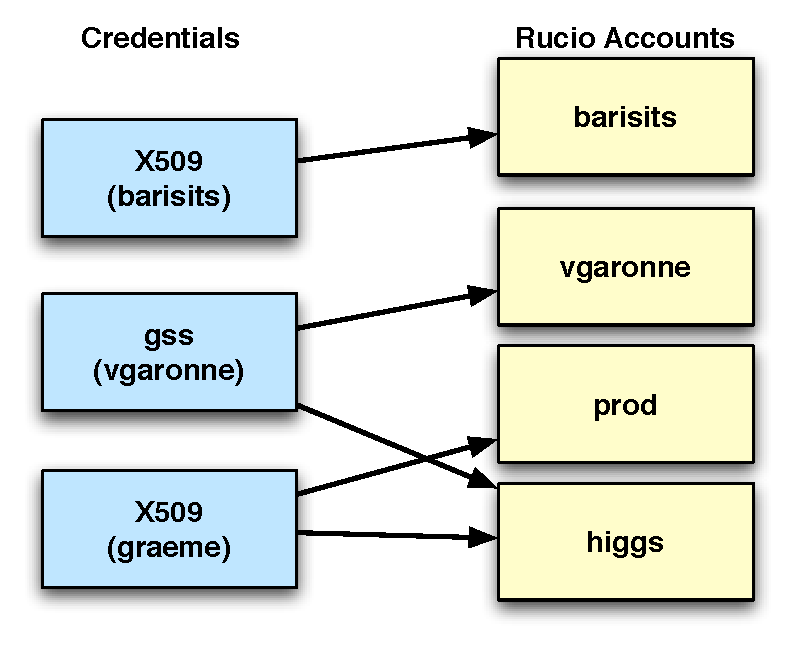
\includegraphics[width=200pt]{accounts.pdf}
\end{center}
\caption{\label{credentials} Credential to Rucio account mapping}
\end{figure}

\section{Files, Datasets and Containers}
\label{overview_Dataset:dataset}

ATLAS has a large amount of data, which is physically stored in files. For the data management system these files are the smallest operational unit of data (so sub-file operations are not possible). Physicists need to be able to identify and operate on any arbitrary set of files.

Files can be grouped into datasets (a named set of files) and datasets can be grouped into containers (a named set of datasets or, recursively, containers). All three types of names refer to data so the term ‘data identifier set’ (DIS) is used to mean any set of file, dataset or container identifiers. A data identifier is just the name of a single file, dataset or container. The figure below gives an example of an aggregation hierarchy:

\begin{figure}[h]
\begin{center}
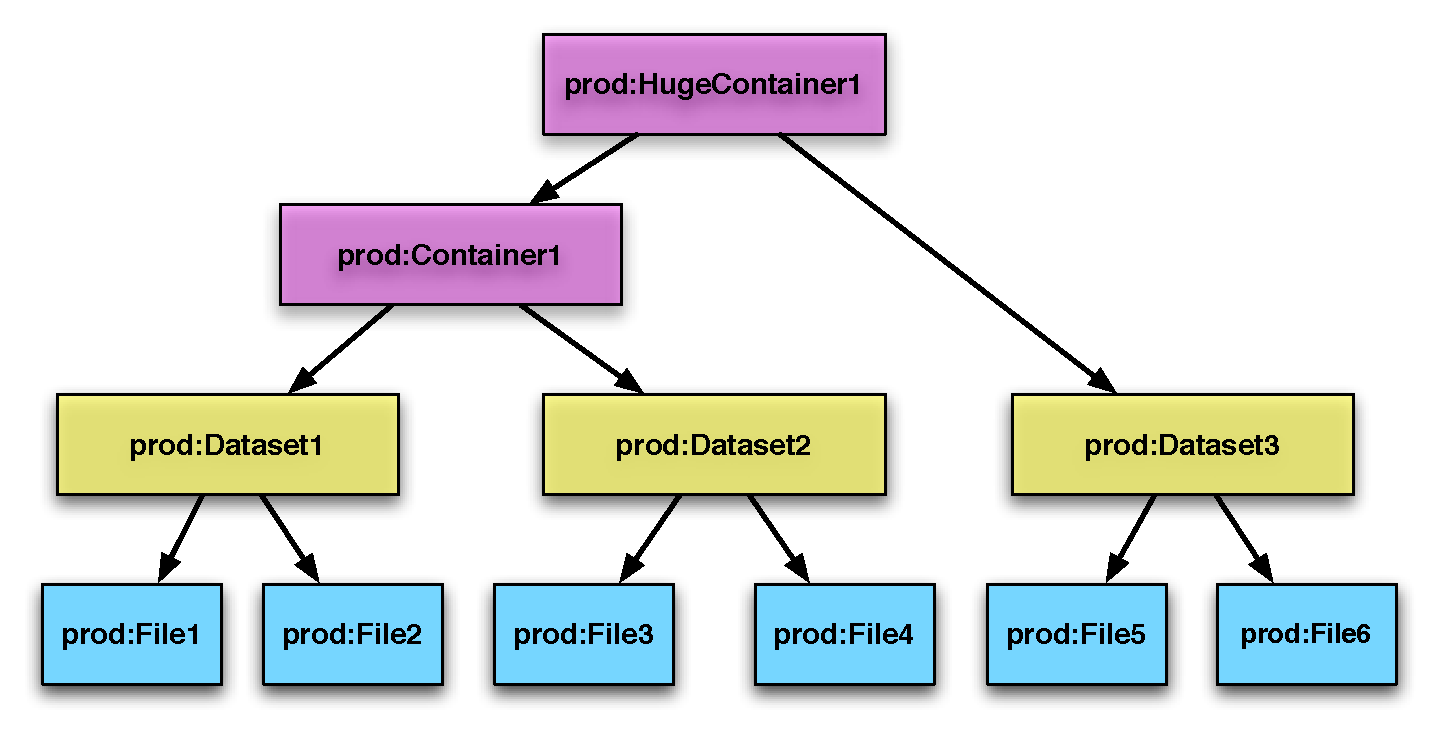
\includegraphics[width=400pt]{aggregation_hierarchy.pdf}
\end{center}
\caption{\label{hierarchy} Rucio aggregation hierarchy}
\end{figure}

\noindent An example of a data identifier set (DIS) is: \{prod:Dataset1, prod:File3, prod:File5\}.

\subsection{Data identifiers and scope}
\label{overview_Dataset:data-identifiers-and-scope}

Files, datasets and containers follow an identical naming scheme which is composed of two strings: the scope and a name. The combination of both is called a data identifier (DI). For instance a file identifier (LFN) is composed of a scope and a file name. The scope string partitions the name space in several sub spaces. The primary use case for this is to have separate scopes for production and individual users.

By default accounts will have read access to all scopes and write access only to their own scope. Privileged accounts will have write access to multiple scopes, e.g., production might use scopes such as mc11, data12\_8TeV, tmp.prod.\footnote{Scopes can be marked as read-only, which will prevent the registration of new data in them.}

Files, datasets and containers are uniquely identified over all time. This implies that an identifier, once used, can never be reused to refer to anything else at all, not even if the data it referred to has been deleted from the system.

\subsection{File, dataset and container status}

\subsubsection{File status}
\label{sec:file-status}

The following status attributes are supported for files:

\begin{itemize}
\item{} \texttt{availability}: LOST, DELETED, AVAILABLE

A file is LOST if there are no known replicas of the file in Rucio, while at the same time at least one account requested a replica; a file is DELETED if no account requested a replica; otherwise the file is AVAILABLE. This is a derived attribute.

\item{} \texttt{suppressed}: TRUE, FALSE

This is a user settable flag. It indicates that the owner of the scope no longer needs the name to be present in the scope. Files that are suppressed (by default) do not show up in search and list operations on the scope. The setting of this flag is subject to conditions, e.g., one can not suppress a file while at the same time requesting it to be replicated somewhere. This flag will be ignored when explicitly listing contents of datasets/containers.
\end{itemize}

\subsubsection{Dataset/Container status}
\label{sec:dataset-container-status}

\label{sec:status}
The dataset/container status is reflected by a set of attributes:

\begin{itemize}
\item{} \texttt{open}: TRUE, FALSE

If a dataset/container is open, content can be added to it. Datasets/Containers are created open and once closed, they cannot be opened again.\footnote{Datasets from which files have been lost can be repaired when replacement files are available, even if Open=False. The replacements need not be binary identical to the lost files.}

\item{} \texttt{monotonic}: TRUE, FALSE

If the monotonic attribute is set, content cannot be removed from an open dataset/container. Datasets/Containers are, by default, created non-monotonic. Once set to monotonic, this cannot be reversed.

\item{} \texttt{complete}: TRUE, FALSE

A dataset/container where all files have replicas available is complete. Any dataset/container which contains files without replicas is incomplete. This is a derived attribute.

\item{} \texttt{suppressed}: TRUE, FALSE

This attribute has the same meaning as for files.
\end{itemize}

\noindent There is no concept of versioning. Adding content to a closed dataset/container is not possible and instead a new dataset/container, with a new identifier, must be created.

\section{Metadata attributes}

Metadata associated with a data identifier is represented using attributes which are key-value pairs. The set of available attributes is restricted. Some metadata attributes are user settable, e.g., physics attributes (number of events, run number, run period, POOL GUID) or production attributes (task ID, job ID). Metadata which is not user settable includes system attributes, such as size, checksum, creation time, etc. For datasets and containers, it is possible that the value of a metadata attribute is a function of the metadata of its constituents, e.g., the total size is the sum of the sizes of the constituents. In this case it is also obviously not possible to assign a value to it.

When appropriate and requested, Rucio will check metadata values for validity, rejecting the attempt to set invalid values. This can be used to ensure that, e.g., POOL GUID is unique and that the Job ID is a positive integer.

The upload of data with incorrect attributes or values will be rejected. Rucio supports searching for files, datasets and containers based on metadata attributes.

\section{Rucio Storage Element}
\label{overview_Rucio_Storage_Element:rucio-storage-element}

A Rucio Storage Element (RSE) is a repository for physical files. It is the smallest unit of storage space addressable within Rucio. It has an unique identifier and a set of properties such as:

\begin{itemize}
\item supported protocols, e.g., file, https, srm
\item quality of service; storage type, e.g., disk, tape
\item physical space properties, e.g., used, available, non-pledged
\item a weight value, used for data distribution (see section \ref{sec:replica-rules})
\item a threshold for deletion (see section \ref{sec:Datadeletion})
\end{itemize}

\noindent A set of RSEs can be identified directly by enumeration of their names, or indirectly by a boolean expression over their attributes. Attributes are key-value pairs, e.g., CLOUD=UK, Tier=1, T2D=True, MoUShare=15. A key whose value is ‘True’ is equivalent to a tag. RSE attributes are used to manage data with replication rules (see section \ref{sec:replica-rules}).

Physical files stored on RSEs are identified by their Physical File Name (PFN). The PFN is a fully qualified path identifying a replica of a file. PFNs may take the form of file names, URIs, or any other identifier meaningful to a Rucio Storage Element. The mapping between the LFN and the PFN is a deterministic function of the LFN, RSE and protocol.

Normally the upload to an RSE and the registration of a replica is a single operation. For trusted users, like the Tier-0 and PanDA production systems, it is possible to register a replica uploaded independently.

\section{Permission model}
\label{overview_Permission_model:permission-model}

Rucio assigns permissions to accounts. Permissions are boolean flags designating whether an account may perform a certain action. For example, the check of the permission to add an account for the rucio administrative account will return true.

\section{Replica management}
\label{overview_Replica_management:replica-management}

\subsection{Replica Rules}
\label{sec:replica-rules}

Replica management is based on replication rules defined on data identifiers. Replication rules defined on datasets or containers will affect all contained datasets, containers and files (either directly or recursively), including content added to these datasets and containers in the future. A replication rule is owned by an account and defines the minimum number of replicas to be available on a list of RSEs.

Rules may have a limited lifetime and can be added, removed or modified at any time. Rules may specify a grouping policy that controls which files are grouped together at the same RSEs (see section \ref{sec:replica-rules}).

The list of RSEs can be specified with RSE attributes (see section \ref{overview_Rucio_Storage_Element:rucio-storage-element}). RSE attributes are resolved at rule creation time to enumerate target RSEs. Post-facto changes to RSE attributes will not affect current replication rules.

Sample replication rules are given below (some parameters are optional, a value in [] denotes usage of the default value):

\begin{minipage}{12cm}
\begin{tabular}{c c c p{2cm} c c c}
\toprule
\textbf{Account} & \textbf{Copies} & \textbf{Data Identifier} & \textbf{RSEs} & \textbf{Weight} & \textbf{Lifetime} & \textbf{Grouping\footnote{See section \ref{sec:file-replica-grouping} }} \\
\midrule
prod & 1 & atlas:container3 & Site=CERN & [MoU] & [No] & All \\
prod & 2 & prod:container1 & Tier=1 & [MoU] & [No] & [Dataset] \\
mario & 1 & mario:container2 & (Cloud=US AND Tier=2) OR Site=CERN & [MoU] & 2013-01-01 & [Dataset] \\
luc & 2 & graeme:file1 & Cloud=UK AND T2D\footnote{This is interpreted as T2D=True.} & No & [No] & None \\
\bottomrule
\end{tabular}
\end{minipage}

As transferring a file to a site can fail, a replication rule has a state to reflect its status:

\begin{enumerate}
\item[] \texttt{satisfied} -- rule is fulfilled by current replicas
\item[] \texttt{replicating} -- not all replicas are made for this rule
\item[] \texttt{stuck} -- replication attempts for at least one replica have failed and have reached an attempt limit
\item[] \texttt{suspended} -- a manually set status, indicating that no further attempts should be made to satisfy the rule
\end{enumerate}

Rucio processes the replication rule(s) and creates replica locks to satisfy the rule(s) and prevent deletion of the replicas. A replica lock is defined for a replica on a specific RSE. It is owned by the account which issued the replication rule. Rucio will record the relationship between the replication rules and replica locks so that the correct locks can be removed when a replication rule is deleted.

A replication rule can generate a data transfer prior to the replica lock being satisfied. Rucio will only create the minimum set of necessary transfer primitives to satisfy all rules. If the weighting option of the replication rule is used, the choice of RSEs takes their weight into account.

For example, \texttt{vgaronne:Dataset1 = \{File1, File2\}} with the replication rule \texttt{'vgaronne: 2 replicas @ Tier=2'} is resolved into two replica locks for each file of the dataset:

\begin{itemize}
\item[] \texttt{vgaronne: File1 @ LMU}
\item[] \texttt{vgaronne: File1 @ MANCHESTER}
\item[] \texttt{vgaronne: File2 @ LMU}
\item[] \texttt{vgaronne: File2 @ MANCHESTER}
\end{itemize}

If Rucio encounters failures when transferring files, it will apply a configurable policy to determine how to proceed. This policy can specify a retry strategy, whether alternative sites can be used and when the rule will be considered stuck.

\subsection{File replica grouping}
\label{sec:file-replica-grouping}

If the file content of a dataset is very widely distributed across many sites this will maximise the CPU resources that can be used to process this data. If the files are concentrated at one site this will be optimal for processing which requires the use of many files at once (e.g., merging and archiving to tape).

Rucio uses the dataset/container hierarchy to control how files are grouped together at sites. Rucio offers three levels of grouping, which will affect how the file replicas in a hierarchy are grouped:
\begin{enumerate}
\item[] \texttt{all} -- All files will be replicated to the same RSE.
\item[] \texttt{dataset} -- All files in the same dataset will be replicated to the same RSE; different datasets will be spread maximally over all allowed RSEs. This is the default.
\item[] \texttt{none} -- Files will be completely spread over all allowed RSEs without any grouping considerations at all.
\end{enumerate}

To illustrate this consider the following dataset hierarchy:

\begin{figure}[h]
\begin{center}
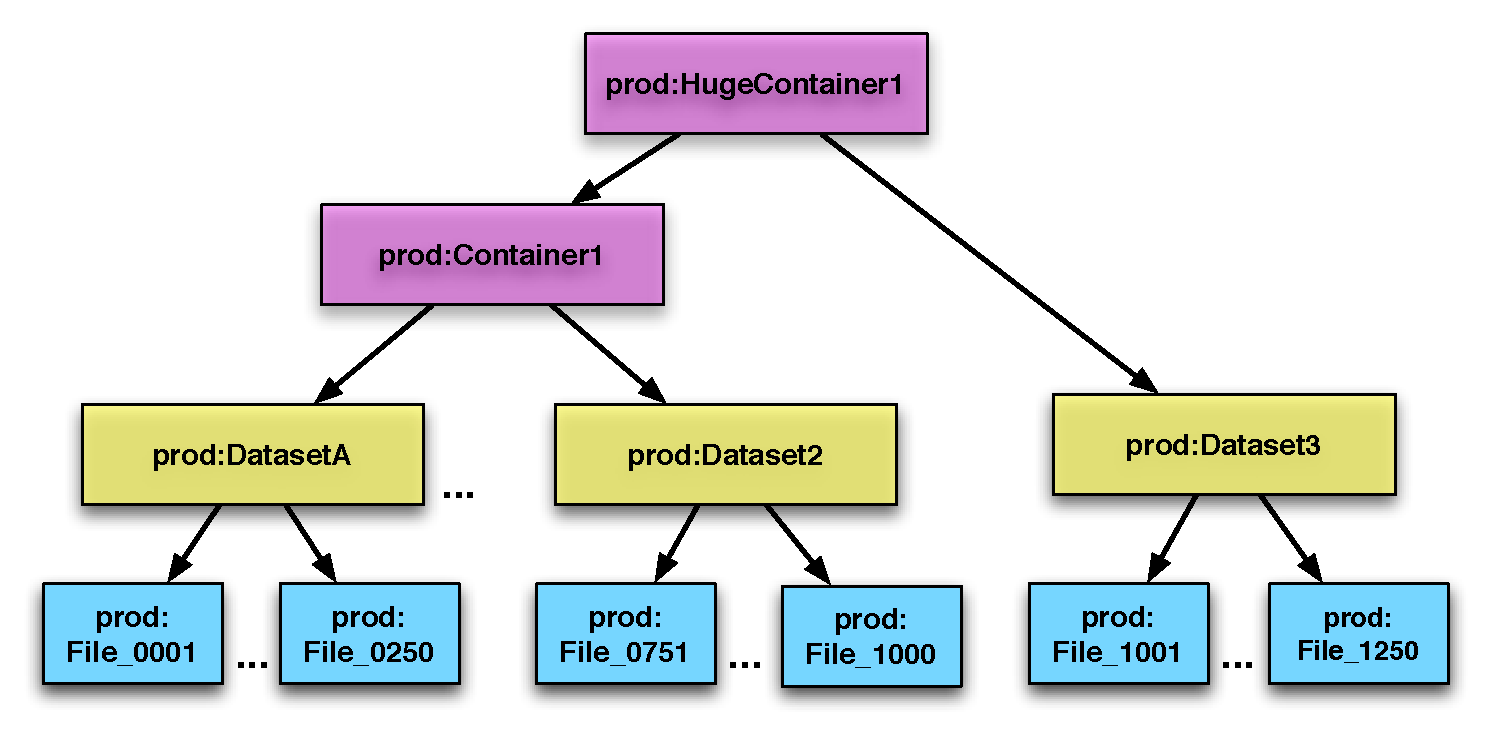
\includegraphics[width=400pt]{dataset_hierarchy.pdf}
\end{center}
\caption{\label{datasethierarchy} Rucio dataset hierarchy with grouping}
\end{figure}

There are 1250 files organised in 5 datasets:
\begin{itemize}
\item[] \texttt{prod:DatasetA = \{prod:File\_0001, \ldots, File\_0250\}}
\item[] \texttt{prod:DatasetB = \{prod:File\_0251, \ldots, File\_0500\}}
\item[] \texttt{prod:DatasetC = \{prod:File\_0501, \ldots, File\_0750\}}
\item[] \texttt{prod:DatasetD = \{prod:File\_0751, \ldots, File\_1000\}}
\item[] \texttt{prod:DatasetE = \{prod:File\_1001, \ldots, File\_1250\}}
\end{itemize}

Some datasets are aggregated into a container:
\begin{itemize}
\item[] \texttt{prod:Container1 = \{prod:DatasetA, prod:DatasetB, prod:DatasetC, prod:DatasetD\}}
\end{itemize}

The container \texttt{prod:Container1} and dataset \texttt{prod::DatasetE} are aggregated into a bigger container:
\begin{itemize}
\item[] \texttt{prod:HugeContainer1 = \{prod:Container1, prod:DatasetE\}}
\end{itemize}

If a replication rule is specified on \texttt{prod:HugeContainer1}, specifying that \texttt{all} grouping should be used, then Rucio will replicate all files belonging to \texttt{prod:HugeContainer1 (prod:File\_0001 \dots File\_1250)} to the same RSE.

If a replication rule with \texttt{dataset} grouping is specified on \texttt{prod:HugeContainer1}, then Rucio will spread the datasets as much as possible over the allowed RSEs, but keep all the files in each dataset at the same RSE.\footnote{Assuming that multiple RSEs are allowed by this rule - specifying a single RSE obviously negates grouping}

If a replication rule with \texttt{none} grouping is specified on \texttt{prod:HugeContainer1}, then Rucio will replicate all files belonging to the datasets to individually random selected RSEs.

Intermediate grouping options, e.g., by specifying a replication rule on \texttt{prod:HugeContainer1}, but only grouping all of the content of \texttt{prod:Container1} together are not supported. To achieve this an individual replication rule has to be specified on \texttt{prod:Container1} with \texttt{all} grouping.

Clients should ensure that their dataset/container hierarchies, in particular the definition of the datasets, are created in such a way as to provide suitable file groupings for further data processing.

\subsection{Subscription}
\label{sec:Subscription}

Subscriptions generate replication rules based on matching particular metadata at registration time. Subscriptions are owned by an account and can only generate rules for that account. Subscriptions do not have a lifetime and need to be removed when no longer required. The lifetime of the generated replication rules can be expressed in a relative way. An example of a subscription is given below:

\bigskip

\begin{tabular}{l p{11cm}}
\toprule
\textbf{Attribute} & \textbf{Value} \\
\midrule
Owner & tzero \\
Match & project=data12\_8TeV AND dataType=RAW AND stream=physics\_* AND DIType=dataset \\
Rule & 1@Site=CERNTAPE; 1@T1TAPE; 1@T1DISK until NOW+90days; grouping=dataset \\
\bottomrule
\end{tabular}

\subsection{Data deletion}
\label{sec:Datadeletion}

In case a replica on a particular RSE has no associated replica locks anymore it can be deleted. Locks disappear when users decrease the number of desired replicas in their replica rules, or the whole rule altogether.

\section{Accounting and quota}
\label{overview_Accounting_and_quota:accounting-and-quota}

Accounting is the measure of how much resource, e.g., storage, an account has used as a consequence of its actions. Quota is a policy limit which the system applies to an account for some resource.

For storage accounting, Rucio accounts will only be charged for the files on which they have set replication rules. The accounting is based on the number of replicas an account requested, not on the number of physical replicas in the system. Accounting and quota calculations use the replica locks generated from replication rules. Quotas are constraints on the replica locks, based on limits set per account.

For example, the GROUPDISK RSE tag could be translated into the following RSE list:\\CERN\_GROUPDISK, BNL\_GROUPDISK, GLASGOW\_GROUPDISK.

\bigskip

\begin{tabular}{l p{9cm} p{2cm}}
\toprule
\textbf{Account} & \textbf{RSE list} & \textbf{Limit (TB)} \\
\midrule
user.vgaronne & CERN\_USERDISK & $< 1$ \\
group.phys-higgs & GROUPDISK AND NOT GLASGOW\_GROUPDISK & $< 30$ \\
group.phys-higgs & CERN\_GROUPDISK & $< 20$ \\
group.phys-higgs & BNL\_GROUPDISK & $< 20$ \\
group.phys-higgs & GLASGOW\_GROUPDISK & $< 100$ \\
\bottomrule
\end{tabular}

\bigskip

\noindent The account user.vgaronne has a quota of 1TB at CERN\_USERDISK. The account group.phys-higgs has an overall quota of 30TB on all GROUPDISK RSEs, excluding GLASGOW. CERN and BNL have an additional protection that group.phys-higgs cannot use more than 20TB on each site, despite the global quota. GLASGOW provides explicitly a quota of 100TB and is excluded from the GROUPDISK quota.

\section{Notifications}
\label{overview_Notifications:notifications}

External applications can require to synchronize on events relative to data availability and can subscribe to particular events, e.g. dataset state changes. Then Rucio will publish a messages to an external application when it detects these events.

\section*{Acknowledgments}
\label{Acknowledgments:acknowledgments}
We express our gratitude to our ATLAS colleagues for their help and patience when we explored requirements and use cases, especially: Markus Elsing, Beate Heinemann, Jamie Boyd, Jonas Strandberg, Solveig Albrand, Torre Wenaus, Rodney Walker, Tadashi Maeno, Paul Nilsson, Simone Campana, Johannes Elmsheuser, Daniel Van Der Ster, Junji Tojo, Ikuo Ueda, Borut Kersevan, Stephane Jezequel and Cedric Serfon.

We also thank Philippe Charpentier, Costin Grigoras, Simon Metson, Latchezar Betev, and Pablo Saiz for their input and ideas about the different distributed data management system of each LHC experiment, and their patience when answering our questions.

\newpage

\label{rucio:appendices}

\section*{Appendix A. Key concepts: Comparison matrix DQ2 vs. Rucio}
\label{Comparison_matrix:key-concepts-comparison-matrix-dq2-vs-rucio}
\begin{tabular}{l l p{5cm} }
\toprule
\textbf{
Features
} & \textbf{
DQ2
} & \textbf{
Rucio
}\\
\midrule
File identifier & GUID/LFN & Scope + name (DI) \\
Dataset identifier & DUID/DSN & Scope + name (DI) \\
Container identifier & CUID/CNT & Scope + name (DI) \\
Versioning & Yes & No \\
Namespace & Global/Flat & Scoped  \\
File aggregation & Dataset & Dataset  \\
Dataset aggregation & Container & Container  \\
Container aggregation & No  & Container  \\
Unique PFN & No & Yes \\
Overlapping dataset & Yes & Yes \\
Storage Element Groups & No & Yes \\
Storage Element Attributes & No & Yes \\
Quota support & Group & Account (Group/User) \\
Replica grouping & Strict & Best effort \\
Replica Lifetime & Yes & No \\
Metadata namespace and support & System defined, Data placement & System defined, Physics, Production, Analysis, Data placement \\
Data discovery unit & Wildcard string matching & Metadata, dataset/container hierarchy\\
Data operation unit &Dataset & Dataset, File, Container (DIS) \\
Multiple replica ownership & No & Yes \\
Dynamic placement & No & Yes \\
Replication rule support & No & Yes \\
Hidden data & Yes & Yes \\
Reuse of dataset name & No & No (but possibility to resuscitate dataset) \\
Notifications & Yes & Yes \\
Fine-grained accounting & Partially & Yes \\
\bottomrule
\end{tabular}

\newpage
\section*{Appendix B. Acronyms and Abbreviations}
\label{Acronyms_and_Abbreviations:acronyms-and-abbreviations}
\begin{description}
\item[{LFN}] Logical File Name.
\item[{DI}] Data Identifier.
\item[{DIS}] Data Identifier Set.
\item[{PFN}] Physical File Name.
\item[{RSE}] Rucio Storage Element.
\item[{URI}] Uniform Resource Identifier.

\end{description}

\end{document}
